\chapter{Visualisierung}
\label{chap.vis}

%PreviewVersion
%\red[TODO:\\
%Ergänzung von Zusatzinformationen noch etwas ausführlicher?\\
%Karte einblenden implementiert?\\
%]

Sobald die aktuelle Position des \kps{s} innerhalb der Umgebung ermittelt wurde kann die Visualisierung der gewünschten Zusatzinformationen basierend auf den Modelldaten (siehe \kapitel{chap.modeldata}) erfolgen. Dieses Kapitel beschreibt das Vorgehen um die ausgewählten Modelldaten mittels des Projektors perspektivisch korrekt in die Umgebung zu projizieren.\\
Zunächst ist die Visualisierung der Modellumgebung und die Ermittlung der Pose des Projektors innerhalb dieser erforderlich. Anschließend erfolgt die Simulation der Projektorsicht durch eine perspektivische Transformation. Die Perspektive wird dabei ausgehend von einem Kameramodell generiert, da der Projektor wie in \abschnitt{chap.kinect} beschrieben als inverse Kamera betrachtet werden kann.\\
Abschließend werden basierend auf der simulierten Perspektive Bilddaten generiert, welche mittels des Projektors für den Anwender und Beobachter innerhalb der realen Umgebung visualisiert werden.

\section{Visualisierung der Modelldaten}
Die Modellumgebung und die Modellobjekte bilden die Grundlage der visuellen Zusatzinformationen die dem Anwender bereitgestellt werden sollen. \\
Um die perspektivische Darstellung zu ermöglichen ist zunächst die gesamte Szene durch die Modelldaten abzubilden. Aufbauend auf der in \kapitel{chap.modeldata} beschriebenen Datenstruktur kann eine Szene erstellt oder geladen und anschließend modifiziert werden. Um eine gerenderte\footnote{Rendern bezeichnet das Ableiten eines Bildes aus virtuellen räumlichen Daten indem die Perspektive eines Beobachters simuliert wird. Dabei können sowohl Lichtverhältnisse als auch Materialeigenschaften berücksichtigt werden um realistische Darstellungen zu erzeugen.} Abbildung der dreidimensionalen Modellszene zu erzeugen wird die Visualisierungsbibliothek VTK (\kapitel{chap.vtk}) verwendet. \abb{fig.modscene} zeigt die Darstellung eines Ausschnitts der Modellszene innerhalb des Visualisierungsbereiches der grafischen Benutzeroberfläche.\\

\begin{figure}[!ht]
	\begin{center}
		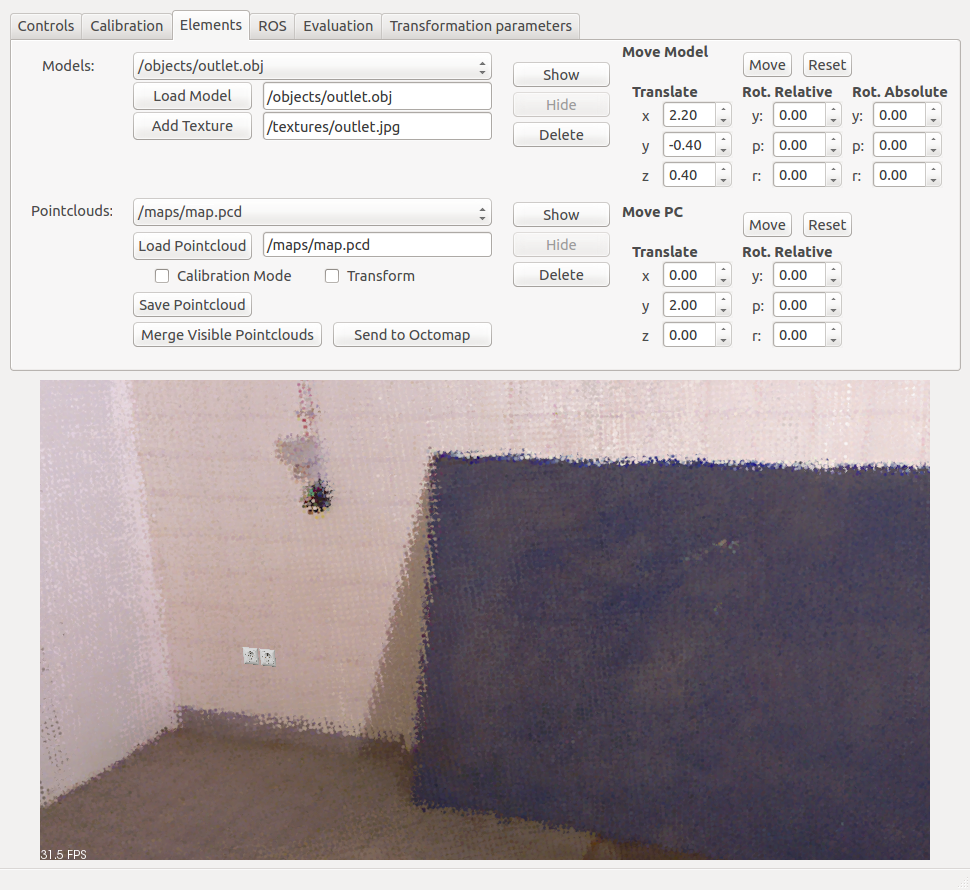
\includegraphics[scale=0.25]{gui}
		\caption{Modellumgebung und Modellobjekte abgebildet innerhalb der grafischen Benutzeroberfläche}
		\label{fig.modscene}
	\end{center}
	%\vspace*{-8mm}
\end{figure}

%PreviewVersion
%\red[CAD-Modell oder Punktwolke? Textur wahrscheinlich schlecht abzubilden!?\\]

Die grafische Benutzeroberfläche ermöglicht die individuelle Positionierung und Ausrichtung aller Elemente. Es werden dadurch die Posen der Objekte und der Umgebung definiert und damit die Transformationen der Modellobjekte $\tmat{0}{Obj}$ und der Modellumgebung $\tmat{0}{Env}$ bezüglich des globalen Koordinatensystems eindeutig festgelegt.\\
Da die für die Lokalisation verwendete Karte aus den Daten der Modellumgebung erzeugt wurde, gilt:

\begin{equation}
\ks{Env} = \ks{M}
\end{equation}

Die Transformation $\tmat{0}{Env}$ ist damit äquivalent zu der Transformation zwischen Karte und globalem Koordinatensystem $\tmat{0}{M}$ und wird deshalb in allen weiteren Ausführungen über diese beschrieben.\\
%PreviewVersion
%Der Zusammenhang zwischen den Koordinaten der Modellumgebung und der Karte der Lokalisation wäre bei einer Veränderung der Pose nicht mehr gegeben und würde zu einem Fehler in der späteren Visualisierung führen. \red[Die grafische Benutzeroberfläche enthält die Möglichkeit eine Zuweisung der Modellelemente zu den Gruppen Umgebung und Objekt vorzunehmen, wodurch die Möglichkeiten zur Modifikation der Elemente entsprechend eingeschränkt oder freigegeben werden.]
%\red[ Objekteigenschaft bool static um Zugehörigkeit zur Map bzw. globalen Koordinaten zu signalisieren. Eigentlich irrelevant in dieser Beschreibung oder?\\]
%\red[Bilder für Modellumgebung und Modellobjekte (z.B. Steckdosen, Leitungen)\\]

\section{Ermittlung der Projektorposition}
Durch die in \abschnitt{chap.projcalib} durchgeführte Kalibrierung ist die externe Transformation $\tmat{KPS}{P}$ zwischen den Basiskoordinaten des \kps{s} und dem Projektor bekannt.\\
Die kontinuierlich durchgeführte Lokalisation des \kps{s} bestimmt die Pose innerhalb der Umgebung worüber sich somit auch die Pose des Projektors bestimmen lässt. Ist diese bekannt, kann durch die Kopplung zwischen den Kartendaten der Lokalisation und den verwendeten Modelldaten die Pose des Projektors innerhalb der simulierten Umgebung bestimmt werden:

\begin{equation}
\tmat{M}{P} = \tmat{M}{Odom}\tmat{Odom}{KPS}\tmat{KPS}{P}
\end{equation}

\section{Perspektivische Transformation}
Die perspektivische Abbildung einer 3D Umgebung auf eine 2D Ebene wurde bereits in \kapitel{chap.perspproj} beschrieben. Der Projektor wird eingesetzt um Daten zu visualisieren, welche zwar innerhalb der Modellumgebung, nicht jedoch in der realen Umgebung vorhanden sind.\\
In der Modellumgebung kann der Projektor deshalb als Kamera simuliert werden, wodurch die Abbildung der Perspektive und Visualisierung dieser möglich wird. Die perspektivische Transformation der Modelldaten erfolgt damit basierend auf der durch die Lokalisation bestimmten extrinsischen $\tmat{M}{P}$ und der bei der Kalibrierung ermittelten intrinsischen Transformation $\tmat{SP}{P}$ des Projektors. Die Abbildung der 3D Modellpunkte auf die 2D pixel der simulierten Kamera wird demnach beschrieben durch:

\begin{equation}
\left(\begin{array}{c}
u_P'\\
v_P'\\
w_P'
\end{array}\right)
= \tmat{SP}{P}(\tmat{M}{P})^{-1}\ve{M}{\tilde{P}} = \tmat{SP}{P}\tmat{P}{M} \left(\begin{array}{c}
X_M\\
Y_M\\
Z_M\\
1
\end{array} \right)
\label{eq.proj_trans}
\end{equation}
%s \cdot \ve{SP}{\tilde{p}} = \tmat{SP}{P}(\tmat{M}{P})^{-1}\ve{M}{\tilde{P}} = \tmat{SP}{P}\tmat{P}{M}\ve{M}{\tilde{P}}

Der durch die Transformation des homogenen 3D-Punktes ermittelte Vektor $[u_P',v_P',w_P']^T$ enthält dabei drei Einträge, welche den in \eq{eq.persp_abb} eingeführten Skalierungsfaktor $s$ enthalten. Um die korrekten Pixelkoordinaten zu ermitteln ist deshalb die Umrechnung der Darstellung des homogenen 2D-Punktes auf einen inversen Streckungsfaktor von $w=1$ erforderlich. Die Pixelkoordinaten des Projektorbildes ergeben sich damit zu:

\begin{equation}
\left(\begin{array}{c}
u_P\\
v_P
\end{array}\right)
=
\left(\begin{array}{c}
\nicefrac{u_P'}{w_P'}\\
\nicefrac{v_P'}{w_P'}
\end{array}\right)
\end{equation}

\abb{fig.projpersp_gui} (a) zeigt die Perspektive des Projektors auf die Modellobjekte innerhalb der Modellumgebung. Bei Generierung der Projektionsabbildung ist zu beachten, dass lediglich die Modellelemente sichtbar sind, die mit dem später projizierten Bild visualisiert werden sollen. Die Modelldaten aller bereits vorhandenen Strukturen werden deshalb wie in \abb{fig.projpersp_gui} (b) gezeigt ausgeblendet, um Überlagerungen von Modelldaten und realen Strukturen zu vermeiden.

%PreviewVersion
%es sei denn, eine   
%optische Bewertung der Projektions- oder Lokalisationsgenauigkeit 
%kann eine Visualiserung der Modellumgebung sinnvoll, um eine  der Überlagerungen von Modelldaten und realen Strukturen zu ermöglichen.

\begin{figure}[!ht]
	\begin{center}
	\subfigure[Projektorperspektive auf Modellumgebung und Modellobjekte]{
		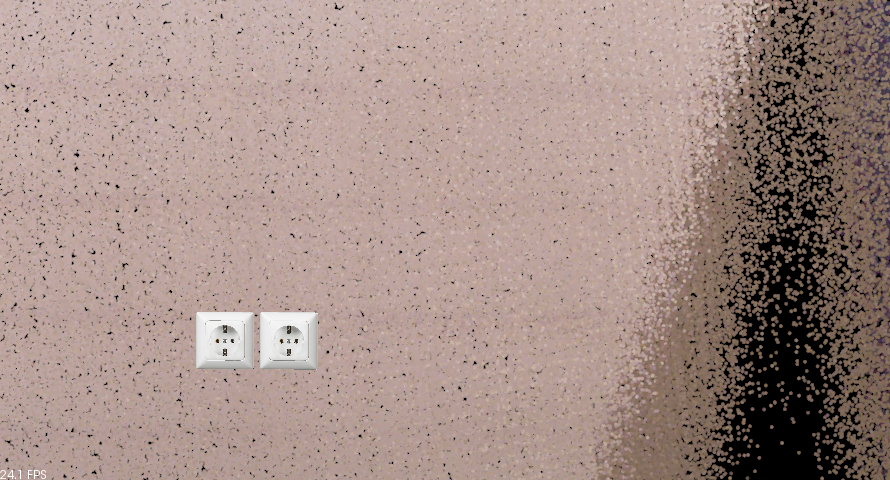
\includegraphics[width=5cm]{proj_persp_incl_map}
	}
	\hspace{5mm}
	\subfigure[Projektorperspektive mit ausgeblendeter Modellumgebung]{
		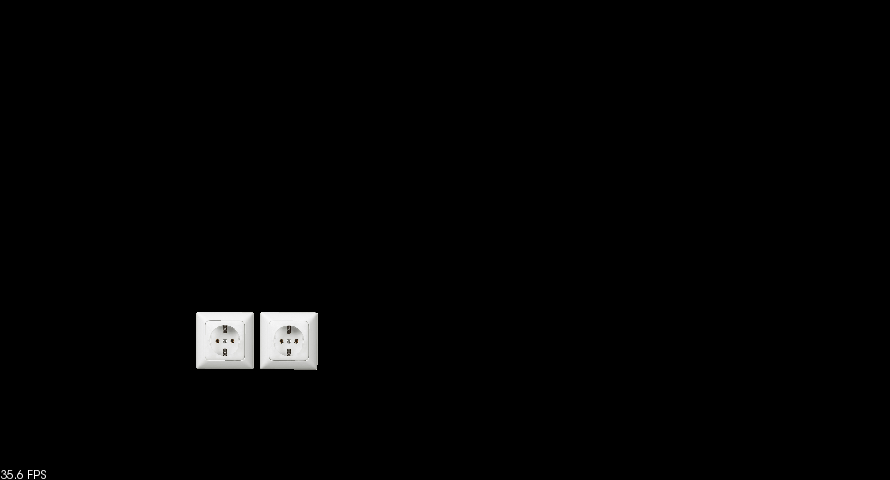
\includegraphics[width=5cm]{proj_persp_no_map}
	}
	\caption{Abbildung der Perspektive des Projektors auf Basis der Modelldaten}
	\label{fig.projpersp_gui}
	\end{center}
	%\vspace*{-8mm}
\end{figure}%
%
%
%\begin{figure}[!ht]
%	\begin{center}
%		\includegraphics[scale=1.0]{perspective_03}
%		\caption{Perspektivische Abbildung der Modelldaten auf die Sensorebene/Pixeldaten des als Kamera simulierten Projektors, grün hervorgehoben das Objekt, das nicht in der Umgebung vorhanden ist aber projiziert werden soll; Rest ausgrauen oder so?}
%		\label{fig.perspproj_vtk}
%	\end{center}
%	%\vspace*{-8mm}
%\end{figure}
%
%\red[Darstellung der Perspektive innerhalb des VTK GUIs]
%
\section{Projektion}
\label{chap.projection}
Nachdem durch die perspektivische Transformation ein Bild der Projektorsicht vorliegt erfolgt die Visualisierung der Modellstrukturen in der realen Umgebung. Da bereits alle nötigen Transformationen des Bildes im Rahmen der perspektivischen Abbildung durchgeführt wurden, kann das vorliegende Bild direkt als Ausgangssignal des Projektors verwendet werden.\\
Die Projektion des virtuellen Modellobjektes in die Umgebung ist in \abb{fig.perspproj} dargestellt. 
%zeigt die Abbildung eines Modellobjektes auf die Bildebene des als Kamera simulierten Projektors. 
Die Bildebene wurde dabei zur Verdeutlichung vergrößert innerhalb des Sichtfeldes des Projektors dargestellt. 

\begin{figure}[!ht]
	\begin{center}
		\includegraphics[width=6cm]{perspective_03}
		\caption{Vorgang der Visualisierung von Modelldaten in der Umgebung auf Basis der simulierten Projektorperspektive}
		\label{fig.perspproj}
	\end{center}
	%\vspace*{-8mm}
\end{figure}

Das projizierte Bild muss dabei nicht auf die Visualisierung der Modellobjekte beschränkt werden. Ergänzend kann das Bild mit weiteren visuellen Informationen versehen werden. \abb{fig.proj_rms} zeigt, wie das Ausgabebild um einem Rahmen erweitert wurde, welcher dem Anwender eine visuelle Rückmeldung über die Güte der Lokalisation basierend auf dem berechneten \red[Quadratischen Mittel der Überdeckungsfehler] (siehe \kapitel{chap.globloc}) gibt.\\

%PreviewVersion
%\red[Projektion der Sicht des Projektors auf das Modell. Ausblenden des Raumes, sodass nur die gewünschten Strukturen dargestellt werden. Alternativ Raummodell als schwarzes Objekt darstellen.\\]

\begin{figure}[!ht]
	\begin{center}
		
\includegraphics[width=5cm]{proj_persp_frame}
		\caption{Visuelle Rückmeldung für den Anwender über die Lokalisationsgüte}
		\label{fig.proj_rms}
	\end{center}
	%\vspace*{-8mm}
\end{figure}

%PreviewVersion
%\red[Karte einblenden!?]